\section{Experiments} 
\label{sec:experiments}


All the pebbling algorithms and heuristics described in the previous sections have been implemented in the hybrid functional and object-oriented programming
language Scala (\url{www.scala-lang.org}) as part of the \skeptik library for proof compression (\url{github.com/Paradoxika/Skeptik}) \cite{Skeptik}.
In order to evaluate them, experiments were executed\footnote{The Vienna Scientific Cluster VSC\nobreakdash-2 
(\url{http://vsc.ac.at/}) was used.} on four disjoint sets of proof benchmarks (Table \ref{tab:benchmarks}). Two of them contain proofs produced by the SAT-solver \texttt{PicoSAT} \cite{Biere_picosatessentials} on unsatisfiable benchmarks from the SATLIB (\url{www.satlib.org/benchm.html}) library. The proofs\footnote{SAT proofs: \url{www.logic.at/people/bruno/Experiments/2014/Pebbling/tc-proofs.zip}} are in the TraceCheck format, which is one of the three formats accepted at the \emph{Certified Unsat} track of the SAT-Competition.
The other two benchmark sets contain proofs produced by the SMT-solver {\veriT} (\url{www.verit-solver.org}) 
on unsatisfiable problems from the SMT-Lib (\url{www.smtlib.org}). These proofs\footnote{SMT proofs: \url{www.logic.at/people/bruno/Experiments/2014/Pebbling/smt-proofs.zip}} are in a proof format that resembles SMT-Lib's problem format and they were translated into pure resolution proofs by considering every non-resolution inference as an axiom.

Figure \ref{fig:SpaceVSLength} relates for each proof the smallest space measure obtained by all algorithms tested on the respective proof and its length in number of nodes. Note that the y-axis, showing the space measures, scale is lower by a factor of 100 than the scale of the x-axis, which displays the proof lengths. On average the smallest space measure of a proof is 44,1 times smaller than its length. This shows the impact that the usage of deletion information together with well constructed topological orders can have. When these techniques are used, on average 44,1 times less memory is required for checking a proof.

\begin{figure}
	\centering
	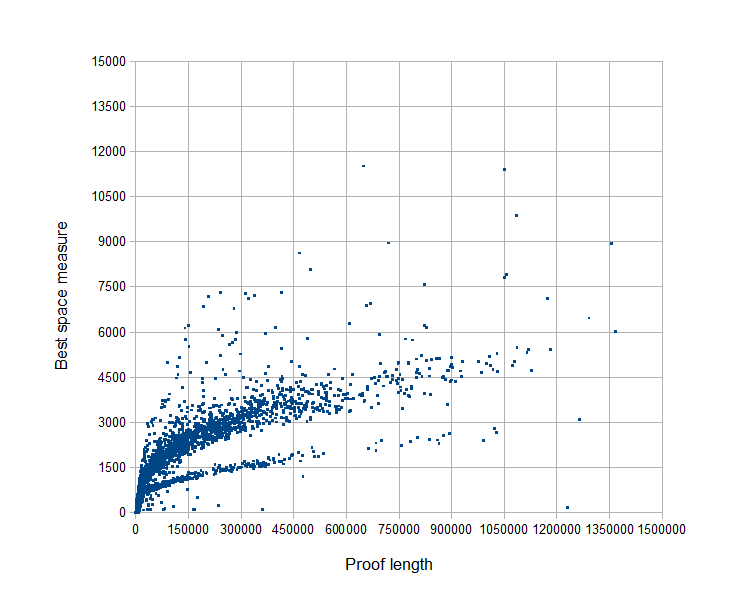
\includegraphics[scale=0.4]{Figures/length_vs_space_2.png}
	\caption{Best space measure compared to proof length}
	\label{fig:SpaceVSLength}
\end{figure}

\begin{figure}
	\centering
	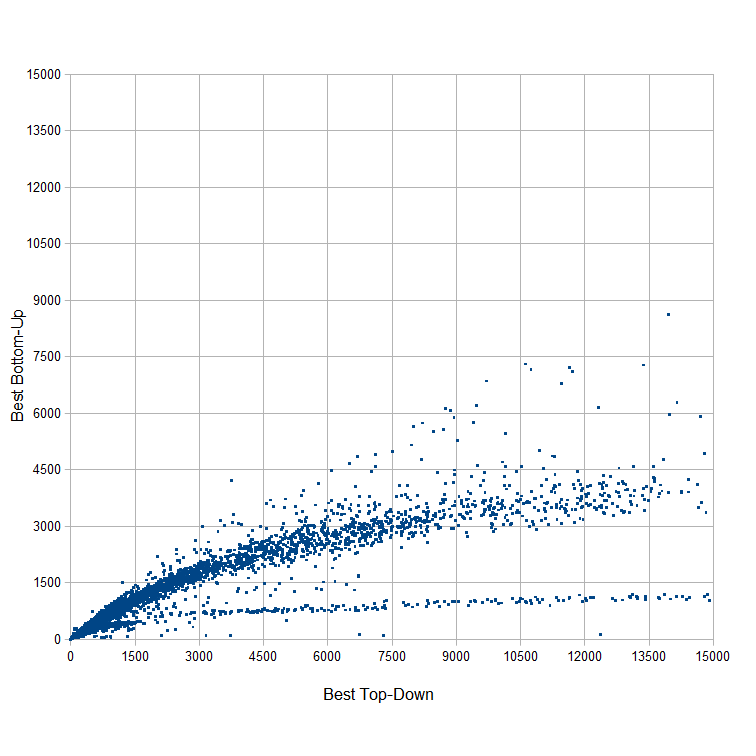
\includegraphics[scale=0.4]{Figures/TD_vs_BU-scatter_min.png}
	\caption{Spaces obtained with best \algo{Bottom-Up} and \algo{Top-Down} heuristics}
	\label{fig:BUvsTD}
\end{figure}


\begin{equation} \label{eq:space}
  \mathit{performance}(f, G, P) = \frac{1}{|P|} * \sum_{\varphi \in P}{\left( 1 -
    \frac{
      s(\varphi,f(\varphi))
    }{
        \mathit{avg}_{g\in G}{s(\varphi,g(\varphi))}
    } \right)
  }
\end{equation}

\begin{table}[tb]
	\centering
	\setlength{\tabcolsep}{8pt}
	\begin{tabular}{|l|c|c|c|}
		\hline
		\textbf{Name} & \textbf{Number of proofs} & \textbf{Maximum length} & \textbf{Average length} \\ 
		\hline \hline
		TRC1 & 2239 & 90756   & 5423   \\ \hline
		TRC2 & 215	& 1768249 & 268863 \\ \hline
    SMT1 & 4187 & 2241042 & 103162 \\ \hline
    SMT2 & 914  & 120075  & 5391  \\ 
		\hline   
	\end{tabular}
	\caption{Proof benchmark sets}
	\label{tab:benchmarks}
\end{table}

\newcommand{\cHline}{\\[-2.5ex] \hline \\[-2.5ex]}
\begin{table}[tb]
\centering
\setlength{\tabcolsep}{8pt}
\begin{tabular}{|l|c|c|c|c|c|c}
\hline
\textbf{Algorithm} & \multicolumn{4}{c|}{\textbf{Relative Performance} (\%)} & \textbf{Speed}\\ 
Heuristic:Method & \textbf{SMT1} & \textbf{SMT2} & \textbf{TRC1} & \textbf{TRC2} & (nodes/ms)\\ 
\hline\hline
Ch:BU & 19,53 & -15,79 & 20,48 & \textbf{88,57} & \textbf{88,55} \\ 
Ch:TD & \textbf{-22,07} & 8,29 & -48,33 & -67,12 & 0,30 \\ \cHline
Lc:BU & \textbf{23,42}& 36,69 & 21,47 & 88,55 & 84,43 \\ 
Lc:TD & -20,88 & 14,20 & -64,07 & \textbf{-110,00} & 1,87 \\ \cHline
Dist(1):BU & & -15,72 & 19,74 & & 21,23 \\ 
Dist(1):TD & & -67,52 & -71,21 & & 0,63 \\ 
Dist(3):BU & & -50,27 & 19,95 & & 0,54\\ 
Dist(3):TD & & \textbf{-74,90} & \textbf{-74,09} & & \textbf{0,08}\\ \cHline
Dc(LC,0.5,1,avg):BU & & 37,39 & 21,83 & & 47,70\\ 
Dc(LC,0.5,7,avg):BU & & 37,78 & 22,05 & & 14,01 \\
Dc(LC,3,1,avg):BU & & 36,86 & 22,02 & & 63,97\\
Dc(LC,3,7,avg):BU & & 34,69 & \textbf{22,55} & & 15,31 \\ 
Dc(LC,0.5,1,max):BU & & 37,31 & 21,76 & & 47,03 \\
Dc(LC,0.5,7,max):BU & & 37,89 & 21,94 & & 15,26 \\
Dc(LC,3,1,max):BU & & 37,33 & 21,79 & & 64,43 \\
Dc(LC,3,7,max):BU & & \textbf{37,96} & 22,13 & & 15,34 \\
%\bottomrule
\hline
\end{tabular}
\caption{Experimental results}
\label{tab:results}
\end{table}

\noindent
Table \ref{tab:results} shows that \algo{Bottom-Up} algorithms construct topological orders with much smaller space measures than \algo{Top-Down} algorithms. This fact is visualized in Figure \ref{fig:BUvsTD}, where each dot represents a proof $\varphi$ and the $x$ and $y$ coordinates show the space of $\varphi$ with the topological orders found by, respectively, the best \algo{Top-Down} and \algo{Bottom-Up} algorithms for $\varphi$. Some other heuristics (not described in this paper) aimed at improving \algo{Top-Down} Pebbling were tested on small benchmark sets, but none showed promising results.

Furthermore, \algo{Bottom-Up} algorithms are also much faster, as can be seen in the last column of Table \ref{tab:results}. This is so because they require fewer comparisons in their heuristic choices. For \algo{Bottom-Up} algorithms, the set $N$ of possible choices consists of the premises of a single node only, and usually $|N| \in O(1)$ (e.g. for a binary resolution proof, $N \leq 2$ always). On the other hand, the set $N$ of currently pebbleable nodes, from which \algo{Top-Down} algorithms must choose, is large (e.g. for a perfect binary tree with $2n -1$ nodes, initially $|N| = n$). For some heuristics, \algo{Top-Down} algorithms could be made more efficient by using, instead of a set, an ordered sequence of pebbleable nodes together with their memorized heuristic evaluations.

Using the \algo{Distance} Heuristic has a severe impact on the speed, which decreases rapidly as the maximum radius increases. With a radius equal to 5, only a few small proofs were processed in a reasonable amount of time.

As expected, the \algo{Decay} Heuristic does improve the results of the underlying heuristic. Note that because of the relative nature of the performance measure and the poor performance of the \algo{Top-Down} algorithms, small performance differences can still be significant. Nevertheless, the performance improvement comes at a high cost in speed.

